90. \begin{figure}[ht!]
\center{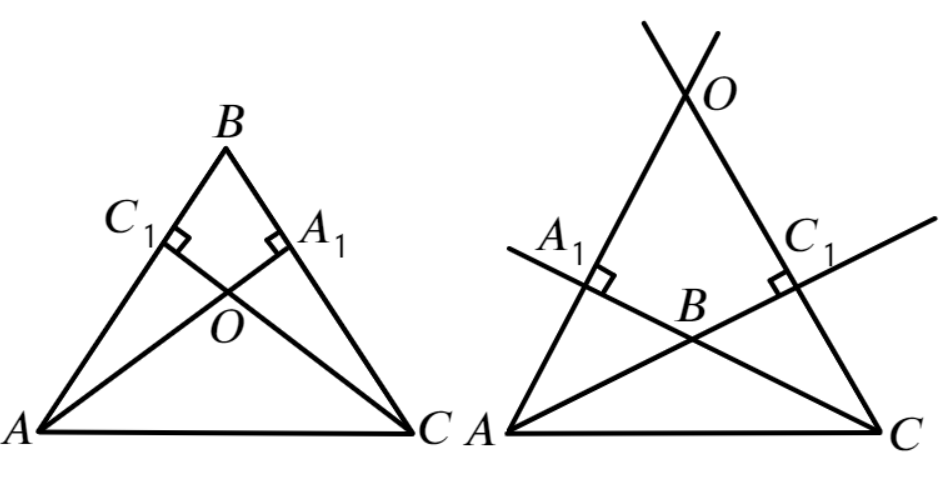
\includegraphics[scale=0.35]{g8-90.png}}
\end{figure}\\
Возможны два случая: треугольник может быть остроугольным или тупоугольным. В обоих случаях необходимо рассмотреть четырёхугольник $C_1BA_1O:$ в первом случае $\angle B =360^\circ-90^\circ-90^\circ-140^\circ=40^\circ,$ а во втором --- $\angle B=\angle C_1BA_1=360^\circ-90^\circ-90^\circ-40^\circ=140^\circ.$ В первом случае мы воспользовались тем, что по определению углом между прямыми называется острый (или прямой) угол.\\
